% Co-authored-by: cherusk <10729954+cherusk@users.noreply.github.com>
\documentclass[11pt,a4paper]{article}
\usepackage[utf8]{inputenc}
\usepackage[T1]{fontenc}
\usepackage{libertine}
\usepackage[libertine]{newtxmath}
\usepackage{amsmath}
\usepackage{graphicx}
\usepackage{xcolor}
\usepackage{booktabs}
\usepackage{subcaption}
\usepackage{titlesec}
\usepackage{tikz}
\usetikzlibrary{arrows.meta,positioning,shapes.geometric}
\usepackage{hyperref}
\usepackage[margin=2.6cm]{geometry}

\title{From Curves to Cascades: Composed Coupling Prediction Among
       Autonomous Agents}
\author{
  Matthias Tafelmeier \\
  Independent Scientist \\
  Hof, Germany \\
  \href{https://orcid.org/0009-0005-7399-5584}{ORCID: 0009-0005-7399-5584}
}
\date{}

\begin{document}
\maketitle

\begin{abstract}
Autonomous agents that share a substrate couple through it, and prior
work established that the resulting edges can be detected and their
response curves measured --- pairwise, with error bars, while the system
is live. This paper asks the next question: do those local measurements
\emph{compose}? Can curves measured on neighboring links, chained
through nonlinear switching elements and summed where paths converge,
predict far-end behavior without walking the whole path? The referee
design keeps the test honest: the pieces that compose into a prediction
and the direct walk that judges it are disjoint measurements, and the
comparison is made against propagated error bars built from the local
noise of each piece. Across the campaign --- four nonlinear chain
seeds, a converging junction, and a live discontinuity relay across
three seeds --- 95 of 97 referee points fall within propagated
two-sigma bars, and the propagated bars are themselves validated: the
hit rate matches the nominal rate without over-rejection. The
measurement horizon is measured, not assumed: roughly two nonlinear
hops at noise $\sigma{=}0.02$, beyond which the far end falls below
the detection floor and composition stops being an economy and becomes
the only remaining door. Boundary rows (a dead planted cell, a
starved-scheduler pair) are reported as receipts, not discarded.
\end{abstract}

\noindent\textbf{Keywords:} active probing, autonomous agents,
multi-agent systems, coupling discovery, composition, response curves,
uncertainty propagation, cascades, system identification, live
systems, complex systems

\section{Introduction}
\label{sec:intro}

When autonomous agents tend the same substrate, each one's parameter
changes travel through the substrate into the others' objectives. The
coupling is real, hidden, and --- as a line of prior work has
established --- measurable without central observers and without
disrupting the system: edges are discovered by guardrail-bounded
probing between the agents themselves~\cite{p1}, and each edge yields a
response curve with per-point error bars, measured by a self-directed
characterization walk~\cite{p2}.

A map of measured edges answers local questions. The operational
questions are not local. \emph{If this agent pushes its parameter, what
happens two hops away?} \emph{Which cascade paths are live, and where
will a change arrive first?} \emph{How much of a far-end shift is
attributable to this sender?} Answering any of them requires the
multi-hop response --- and measuring it directly runs into a wall that
is arithmetic, not engineering: coupling attenuates multiplicatively
along the path while noise does not, so the far end of a deep chain
sinks toward the noise floor. This paper's boundary experiment shows
the wall in numbers: a three-hop nonlinear chain composes to roughly
$0.001$ of the source's span, twenty times below the $\sigma{=}0.02$
floor, and the direct walk there measures faithful flat noise
(\S\ref{sec:results}). Far-end measurement is not slow; past the
horizon it is \emph{vacuous}.

The alternative is to measure neighbors and compose. One hop away, the
signal is strong, the bars are thin, and the measurement is cheap. If
the measured curves compose --- if the response of a relay can be read
off a neighbor's self-map, if converging paths sum, if a discontinuity
predicted from pieces lands where the direct walk later finds it ---
then the reach of the map is the reach of arithmetic rather than the
reach of the probe. And if the error bars compose with the curves, the
prediction carries its own price tag.

This paper tests exactly that, and the contributions are the clauses
of the test:

\begin{enumerate}
\item \textbf{Composition.} Pairwise-measured coupling curves, chained
through nonlinear switching elements (``doors'') and summed at a
converging junction, predict far-end responses without walking the
path: 95 of 97 referee points within propagated two-sigma bars across
chains, junction, and discontinuity rows
(\S\ref{sec:results}).
\item \textbf{Metrology.} The error bars compose too. Local
per-point bars, propagated through the composed stages in quadrature
with local slopes, neither over-reject (the strict test that ignores
the composed side's uncertainty loses four more points) nor dissolve
into vacuity (median referee deviation ${\approx}\,0.3\sigma$). The
composed map prices its own predictions
(\S\ref{sec:referee}).
\item \textbf{Discontinuity.} Composition survives a live threshold:
the predicted far-end step matches the directly measured step
($-0.159$ predicted against $-0.161$ planted, the direct walk landing
on both), and the flip is bracketed between the same two levels the
pieces pin down --- across three seeds
(\S\ref{sec:results}).
\item \textbf{Boundary.} The composition horizon is measured, not
assumed: ${\approx}\,2$ nonlinear hops at $\sigma{=}0.02$. Beyond it
the referee itself goes vacuous --- the honest outcome, reported as a
result (\S\ref{sec:results}).
\item \textbf{Certification.} The two rows run under the final
protocol --- fair lease turn-taking with a visible turn ledger ---
complete all four walkers' maps in a single cell each, with rotation
verified event by event. The scheduler defects that earlier rows
survived are banked as disclosed before-receipts, not hidden
(\S\ref{sec:results}).
\end{enumerate}

The framing is deliberately plain: one method, measured boundaries.
Cascade identification through known blocks is a classical subject;
what is new here is the specific assembly --- distributed, autonomous,
behavioral measurement whose pieces compose with priced uncertainty on
a running system. \S\ref{sec:related} says the classical part first.
All runs carry external identifiers; every figure regenerates from the
retained evidence by a shipped script.

\section{Related Work}
\label{sec:related}

\paragraph{Block-oriented system identification.}
Composing a nonlinear cascade from measured blocks is textbook
material in the Wiener--Hammerstein lineage~\cite{wiener1958,giri2010}:
a system is modeled as static nonlinearities interleaved with linear
dynamics, and each block is identified separately, then composed. We
state this first, before a reviewer does: nothing in this paper's
composition arithmetic is new. What differs is the measurement
condition. Classical block identification assumes one experimenter who
owns the plant, can isolate signals, and pauses the world between
experiments. Here the ``blocks'' are couplings between autonomous
agents that neither own nor see each other; every reading is
attributed by protocol (turn-taking, parking, block design) rather
than by experimental isolation; and the composed prediction is checked
against a second, disjoint measurement taken by the same protocol on
the same running system. System
identification~\cite{ljung1999sid} remains the mature neighbor for
the single-owner quiet case. Passive
methods~\cite{sugihara2012ccm} cannot see through self-generated
exploration noise at realistic budgets, as the detection study
established~\cite{p1}.

\paragraph{Sharing a substrate fairly.}
The measurement protocol serializes probing through leases; when
several walkers contend, the scheduler question is fair sharing.
The turn ledger used here descends from fair queueing --- deficit
round-robin~\cite{shreedhar1995} and the max-min lineage behind
it~\cite{demers1990} --- instantiated at equal weights on lease
acquires instead of packets. \S\ref{sec:results} reports both sides of
this: rows taken under a defective scheduler, and certification rows
taken under the repaired one.

\paragraph{Empirical coupling discovery.}
The space this line of work occupies --- multiple autonomous
experimenters discovering the coupling structure of the live substrate
they act on, with certified quantitative output --- has, to our
knowledge, no other occupant. The relation to causal
inference~\cite{pearl2009causality} is parallel rather than
subordinate: Pearl's experimenter is centralized and hypothesizes a
model; here the experimenters are the coupled nodes themselves, and
the model is measured edge by edge. No novelty claim is made beyond
the assembly.

\section{The Instrument, Briefly}
\label{sec:instrument}

The instrument is unchanged from prior work; the question is new. This
section fixes vocabulary. The substrate is a set of nodes, each
mapping parameters to objectives through a base function (linear,
polynomial, threshold, saturation); directed edges feed one node's
(noisy) channel value into another's, scaled by a planted strength.
Autonomous agents --- \emph{breeders}, one per node --- walk their
own parameter axis under a push/hold/pause block protocol coordinated
by fencing-token leases: the sender probes a level, receivers park and
hold still, the pause block checks reversibility. Readings are block
medians with error bars from local noise (median absolute deviation);
no response model is fitted anywhere. A self-directed walk chooses its
next level inside the gap where the most structure could still hide,
and retires under a priced stop when every remaining gap could not
hide more than the measurements are uncertain by~\cite{p2}.

Two properties matter for composition. First, curves are
\emph{level-addressed}: a point's address is the total input level at
the measured node, not the knob position that produced it. Second,
every walk banks curves from \emph{all} receivers, so the map of each
sender is complete at retirement --- including the sender's own
self-curve. Both properties earn their keep below; the one referee
miss in the discontinuity family is a single read taken while a
bystander's own dial was off its park position --- a dial-addressed
lookup mis-attributing a correct reading, which level addressing
tolerates.

Multi-walker cells add the scheduler. The final protocol keeps a turn
ledger (per-group acquire counts) and grants the lease to the
walk-pending contender with the fewest turns; certification rows run
under it (\S\ref{sec:cert}). Its lineage is fair
queuing~\cite{demers1990,shreedhar1995}.

\section{The Composition Claim and Its Referee}
\label{sec:referee}

\subsection{The claim}

Let each measured curve be a set of triples $(x, y, \sigma)$: input
level, response, bar. The composition claim is that for a path
$n_1 \to n_2 \to n_3$ through nonlinear elements, the response at
$n_3$ to $n_1$'s level $L$ equals the tail map evaluated at the level
induced by the first hop,
\begin{equation}
\hat{y}(L) \;=\; S_3\bigl(\phi(P(L))\bigr),
\label{eq:compose}
\end{equation}
where $P$ is the measured $n_1{\to}n_2$ piece, $S_3$ the measured
self-map of $n_3$, and $\phi$ the level algebra that converts the
piece's output into the tail map's input address --- in the
discontinuity scenario, $\phi(u) = 50 + 45u$: a channel addition of
$0.45\,u$ at a node parked at $0.5$ lands at the self-map's level
$50 + 45u$. At a converging junction the two path outputs add in the
channel before the tail map is evaluated. The algebra is elementary;
its discipline is \emph{level is level} --- addresses are total input
levels, never knob positions.

\subsection{The referee}

Equation~\eqref{eq:compose} is checkable because the map contains its
own control: the sender's walk banks a \emph{direct} curve to the far
end alongside the pieces. The referee test compares the composed
prediction against this direct walk, point by point:
\begin{equation}
z(L) \;=\; \frac{\lvert y_{\text{direct}}(L) - \hat{y}(L)\rvert}
{\sqrt{\sigma_{\text{direct}}^2(L) + \sigma_{\text{pred}}^2(L)}},
\qquad z < 2 \;\text{certifies.}
\label{eq:referee}
\end{equation}
The design has three teeth. \emph{Disjointness}: the pieces and the
referee are different measurements; a defect in either fails the test
(the starved-scheduler rows below show exactly this). \emph{Priced
uncertainty}: $\sigma_{\text{pred}}$ is propagated from the pieces ---
each stage contributes its local bar and its local slope acting on the
input's bar, combined in quadrature,
\begin{equation}
\sigma_{\text{stage}}^2 = \sigma_{\text{map}}^2(x^\ast) +
\bigl(s_{\text{map}}(x^\ast)\,\sigma_{\text{in}}\bigr)^{2},
\label{eq:prop}
\end{equation}
with bars taken at the bracketing measured levels (the flanks'
maximum) --- conservative by construction. \emph{Planted truth}: the
bench's closed-form responses score every point against ground truth
the agents never see, so piece fidelity and shape are separately
auditable. The referee rule~\eqref{eq:referee} is the single rule
applied to every row of this paper; where a stricter variant (direct
bar only, treating the prediction as exact) changes a count, the
change is reported (\S\ref{sec:metrology}).

Figure~\ref{fig:schematic} fixes the pattern for the discontinuity
scenario: the relay piece and the tail self-map compose into the far-end
prediction; the direct walk judges it.

\begin{figure}[t]
\centering
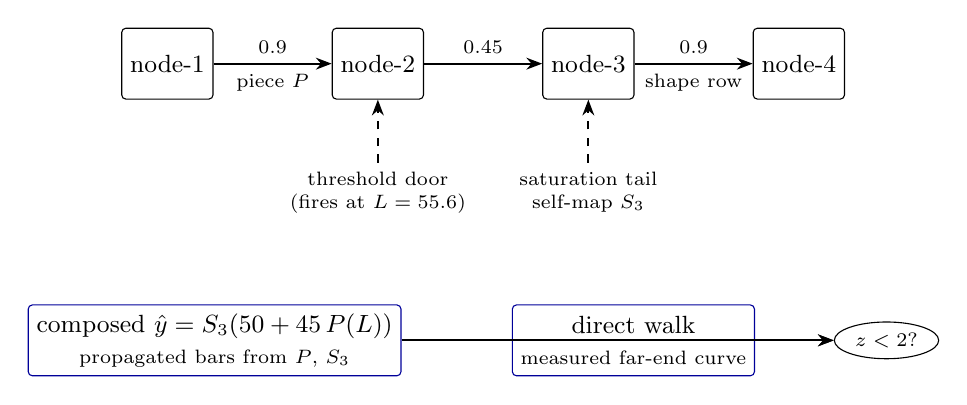
\begin{tikzpicture}[
  node distance=11mm and 15mm,
  box/.style={draw, rounded corners=1.5pt, minimum height=9mm,
              inner sep=3pt, font=\small},
  lbl/.style={font=\scriptsize, align=center},
  arr/.style={-{Stealth[length=2mm]}, thick}]
\node[box] (n1) {node-1};
\node[box, right=of n1] (n2) {node-2};
\node[box, right=of n2] (n3) {node-3};
\node[box, right=of n3] (n4) {node-4};
\draw[arr] (n1) -- node[above, lbl] {$0.9$} node[below, lbl] {piece $P$} (n2);
\draw[arr] (n2) -- node[above, lbl] {$0.45$} node[below, lbl] {} (n3);
\draw[arr] (n3) -- node[above, lbl] {$0.9$} node[below, lbl] {shape row} (n4);
\node[lbl, below=8mm of n2] (door) {threshold door\\ (fires at $L=55.6$)};
\node[lbl, below=8mm of n3] (tail) {saturation tail\\ self-map $S_3$};
\draw[arr, dashed] (door) -- (n2);
\draw[arr, dashed] (tail) -- (n3);
\node[box, below=26mm of n1, xshift=6mm, draw=blue!60!black, align=center] (pred)
  {composed $\hat{y}=S_3(50+45\,P(L))$\\ \scriptsize propagated bars from $P$, $S_3$};
\node[box, right=14mm of pred, draw=blue!60!black, align=center] (direct)
  {direct walk\\ \scriptsize measured far-end curve};
\node[draw, ellipse, inner sep=2pt, right=10mm of direct, font=\scriptsize] (cmp) {$z<2$?};
\draw[arr] (pred) -- (cmp);
\draw[arr] (direct) -- (cmp);
\end{tikzpicture}
\caption{The referee pattern (discontinuity scenario). Pieces measured
by the walkers compose through the level algebra into a far-end
prediction; the same walk's direct curve judges it. Pieces and
referee are disjoint measurements; the comparison is priced by
propagated bars~\eqref{eq:prop}.}
\label{fig:schematic}
\end{figure}

\section{Experimental Design}
\label{sec:design}

\paragraph{The bench as oracle.}
All rows run on the parameterizable substrate of prior
work~\cite{p2}: planted topologies, closed-form responses, Gaussian
noise $\sigma{=}0.02$ per reading, truth invisible to the agents.
Scenarios are chosen to stress one composition structure each:
\emph{door-chain} (a nonlinear door between two saturating stages,
four seeds), \emph{junction-gate} (two converging relay paths into one
tail node), \emph{cliff} (a threshold relay mid-chain whose firing
creates a live discontinuity, three seeds), \emph{poly} (smooth convex
nonlinearity, shape validation), and \emph{depth4} (three cascaded
nonlinear stages --- the boundary probe). Table~\ref{tab:rows} lists
run identifiers.

\paragraph{Pre-flight gate.}
Before any dispatch, the planted far-end span must exceed several
noise bars, and every door's switching condition must be reachable
through the upstream output range. Both checks are one-liners over
the planted forms; the campaign's one dead cell (\S\ref{sec:salvage})
is the receipt that motivates them --- authored before the gate
existed.

\paragraph{Scheduling, disclosed.}
Mid-campaign, multi-walker rows exhibited a lease-starvation defect:
one walker monopolized probe windows and a tail node's self-map
retired at three points. The defect and its fix (the turn ledger of
\S\ref{sec:instrument}) are part of the record: affected rows are
reported with their verdicts \emph{and} their map depths, the
fair-scheduler repair is certified by its own rows, and the two
certification cells of \S\ref{sec:cert} run the final protocol
end-to-end. Runs from before the repair are marked in
Table~\ref{tab:rows}.

\paragraph{Doctrine.}
As in prior work~\cite{p2}: no minimum performance bar; expected
degradation at the map's edge is a result, not a failure; the only
defect signal is the strong-signal/low-noise corner contradicting
itself. Verdicts are recomputed from retained curves, never read from
run badges; verdict tooling is reviewed like engine code (one early
verdict pass had a unit bug that mis-scored a row until repair --- the
receipt is in the run record).

\section{Results}
\label{sec:results}

\begin{table}[t]
\centering
\caption{The composition campaign. Referee = direct walk vs composed
prediction, rule~\eqref{eq:referee}; ``pts'' counts referee points.
Run identifiers are external (GitHub Actions run ids); $\dagger$ =
pre-repair scheduler (disclosed, \S\ref{sec:design}).}
\label{tab:rows}
\small
\begin{tabular}{llll}
\toprule
Row & Run(s) & Referee & Notes \\
\midrule
Linear 3-hop precedent & chain4 bridge cell & --- &
  pred $0.0956$ = measured $0.0956$ vs planted $0.105$ \\
Nonlinear chain, 4 seeds & door-chain s42--45 & 28/28 pts &
  two sequential doors \\
Junction (converging) & 33522428904 & 11/12 pts &
  max $z{=}2.10$ at $L{=}0$; step exact \\
Live discontinuity & 33623243676 & 33/34 pts &
  miss = one off-park read; piece 34/34 \\
\quad certification, s47 & 33968683471 & 11/11 pts &
  piece 11/11, shape 11/11; 4/4 walks \\
\quad certification, s48 & 33974815211 & 12/12 pts &
  piece 12/12, shape 12/12; 4/4 walks \\
Poly shape validation & 33607018911 & 12/12, 12/12 &
  worst $z$ 0.83/0.95; spans 30$\sigma$/18$\sigma$ \\
Dead-plant salvage & 33597128644 & --- &
  piece 18/18; 36 pts no phantom firing \\
Depth boundary & 33558088446 & vacuous &
  3 hops compose to $0.001$ = 20$\times$ below floor \\
\midrule
\multicolumn{4}{l}{\emph{Before-receipts (scheduler defect, excluded from certification)}} \\
Junction, starved & 33634967561$^\dagger$ & 20/22 &
  tail self-map 3 pts; misses localized \\
Junction, starved & 33644675248$^\dagger$ & 14/14 (luck) &
  same defect, clean by chance; excluded \\
Junction, fair-but-thin & 33673988909 & 25/31 &
  turn ledger live, self-map still thin (see text) \\
\bottomrule
\end{tabular}
\end{table}

\subsection{Chains: the anchor rows}
\label{sec:chains}

The door-chain rows are the anchor. Four seeds walk a chain whose
intermediate node is a genuine nonlinear door between saturating
stages; the referee compares the composed two-hop prediction against
the direct walk at every measured level. All 28 referee points across
the four seeds certify within propagated bars; the linear precedent
row bookends the family from the other end --- three linear hops
whose composed prediction ($0.0956$) matches the directly measured
far-end response ($0.0956$) against a planted $0.105$. Composition
holds through smooth nonlinearity, through switching nonlinearity, and
in the linear limit.

\subsection{The junction: composition under superposition}
\label{sec:junction}

Where two paths converge (Figure~\ref{fig:junction}), the composed
input to the tail node is the \emph{sum} of the two path outputs --- a
saturation relay on one path, a threshold relay on the other --- and
the tail's own self-map converts the summed channel level into the
far-end response. The referee certifies 11 of 12 points; the single
miss sits at $L{=}0$ with $z{=}2.10$, on the flat shelf where both
relays are off. Two features deserve the reader's eye in the figure.
The junction map (lower left) is measured by the tail node walking
\emph{its own} dial --- the composition reuses it through the level
algebra, never re-measuring the far end. And the predicted step lands
exactly where the direct walk finds it: the threshold path fires at
the planted $L{=}55.6$, and both prediction and direct curve step
there together.

\begin{figure}[t]
\centering
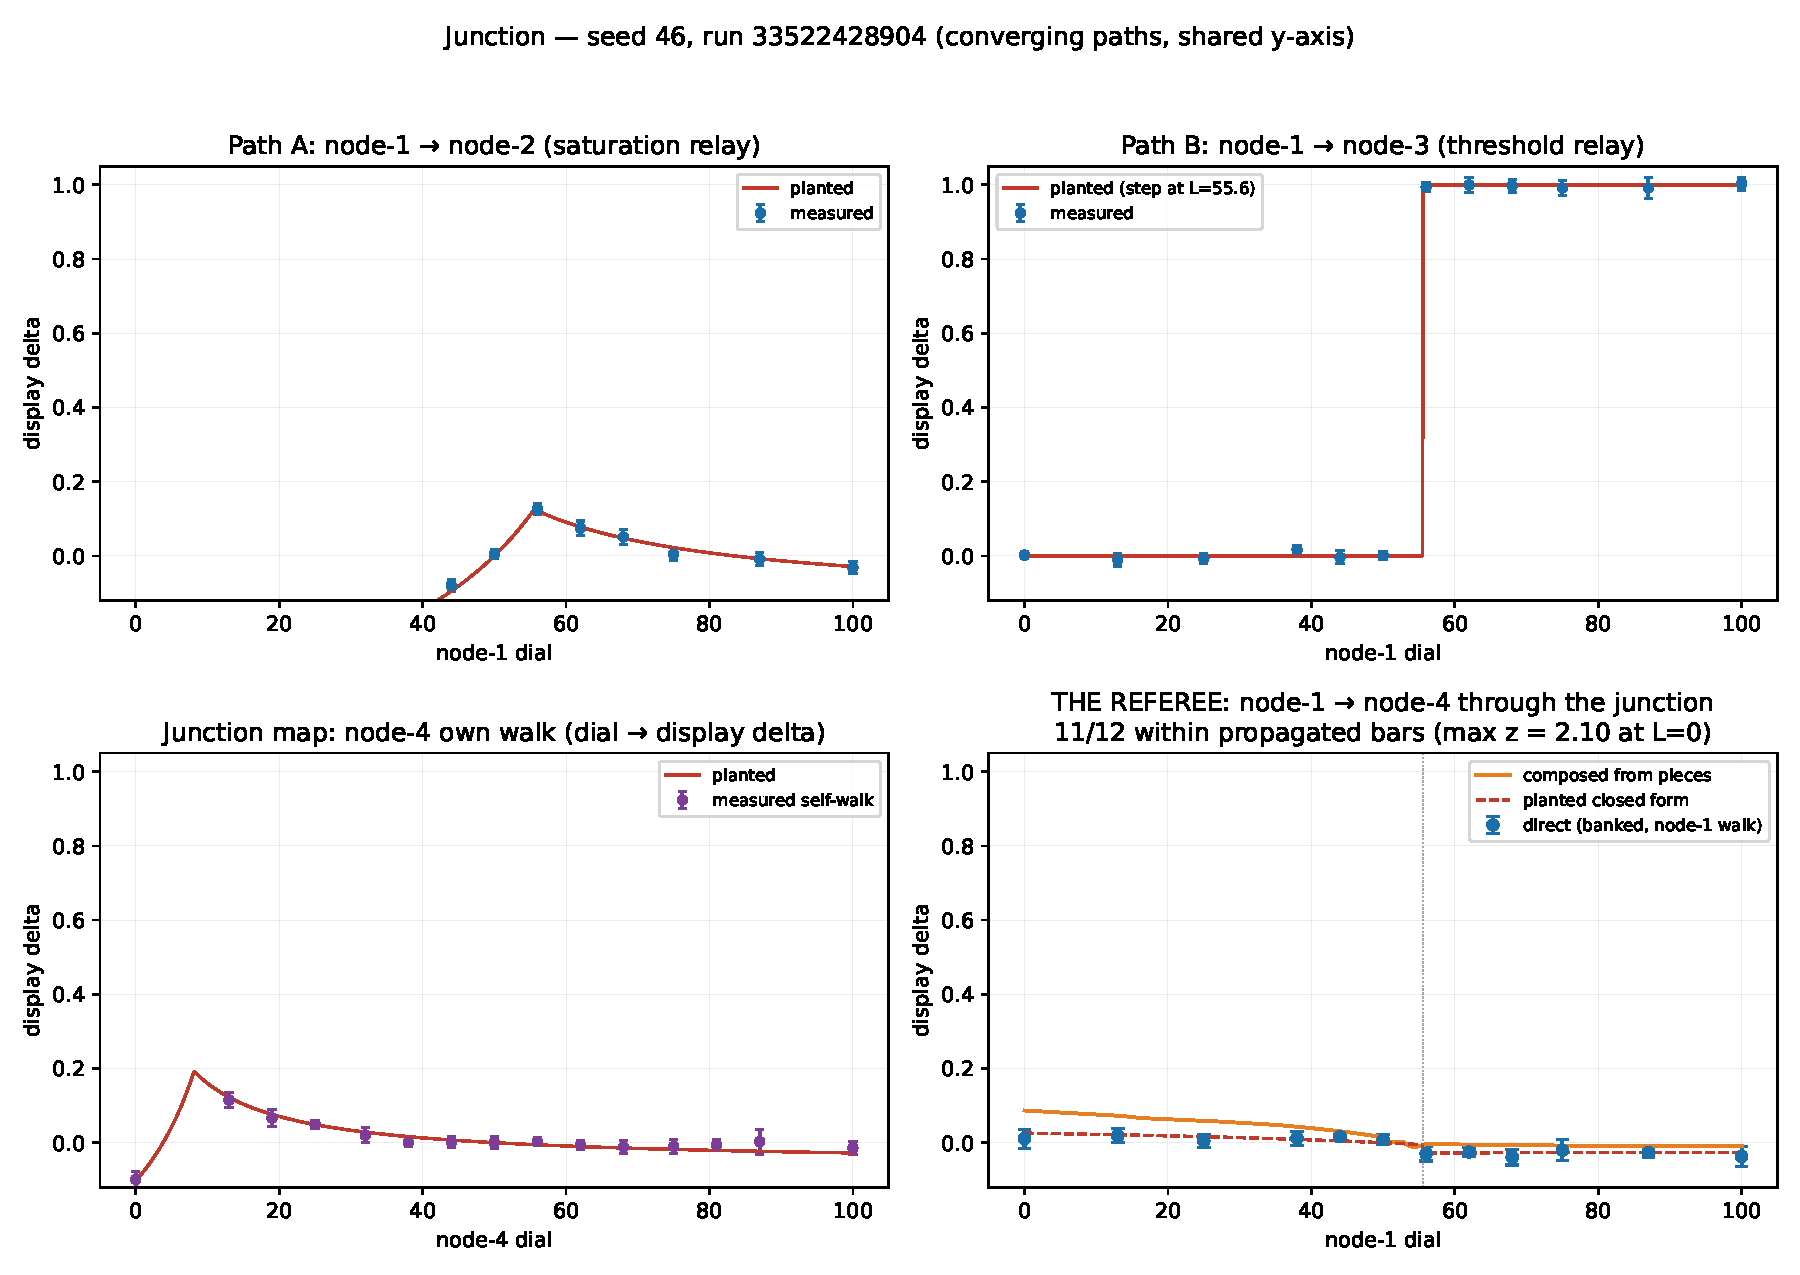
\includegraphics[width=\textwidth]{figures/fig4_junction_s46.pdf}
\caption{Junction row (run 33522428904, seed 46). Top: the two relay
pieces. Bottom left: the tail node's self-walk, reused through the
level algebra. Bottom right: the referee --- direct curve (blue),
composed prediction (orange), planted closed form (dashed red), shared
$y$-axis: the noise floor is one floor.}
\label{fig:junction}
\end{figure}

\subsection{The cliff: composition through a live discontinuity}
\label{sec:cliff}

The cliff scenario places a threshold relay mid-chain: below the
firing level the far end sees nothing; above it, the tail saturation
takes the full relayed step. Composition here is not interpolation ---
the prediction must reproduce a jump \emph{it has never seen at the
far end}, using only the relay piece (measured one hop in) and the
tail self-map (measured by the tail node itself).

Figure~\ref{fig:cliff47} shows a certification cell (seed 47). The
relay piece pins the firing bracket between levels 53 and 56; the
composed prediction steps from the flat shelf to $-0.151$ across the
same bracket; the direct walk lands on it at every level --- 11/11
within propagated bars, far-end step measured at $-0.158$ against a
planted $-0.161$. Seed 48 (Figure~\ref{fig:cliff48}) repeats the cell
under the final protocol: 12/12, step $-0.163$, flip bracketed one
level tighter (54--56). The earlier discontinuity row (33/34) carries
the family's instructive miss: at $L{=}50$ the direct read is
$-0.4995$ --- exactly the tail node's self-curve bottom --- because
one sample was taken while the tail's own dial sat near zero instead
of parked. The reading was \emph{correct} at its true input level; the
curve's dial-addressed label was wrong. The level-addressing
discipline of \S\ref{sec:instrument} is the fix, and the miss is the
receipt that motivated it.

\begin{figure}[t]
\centering
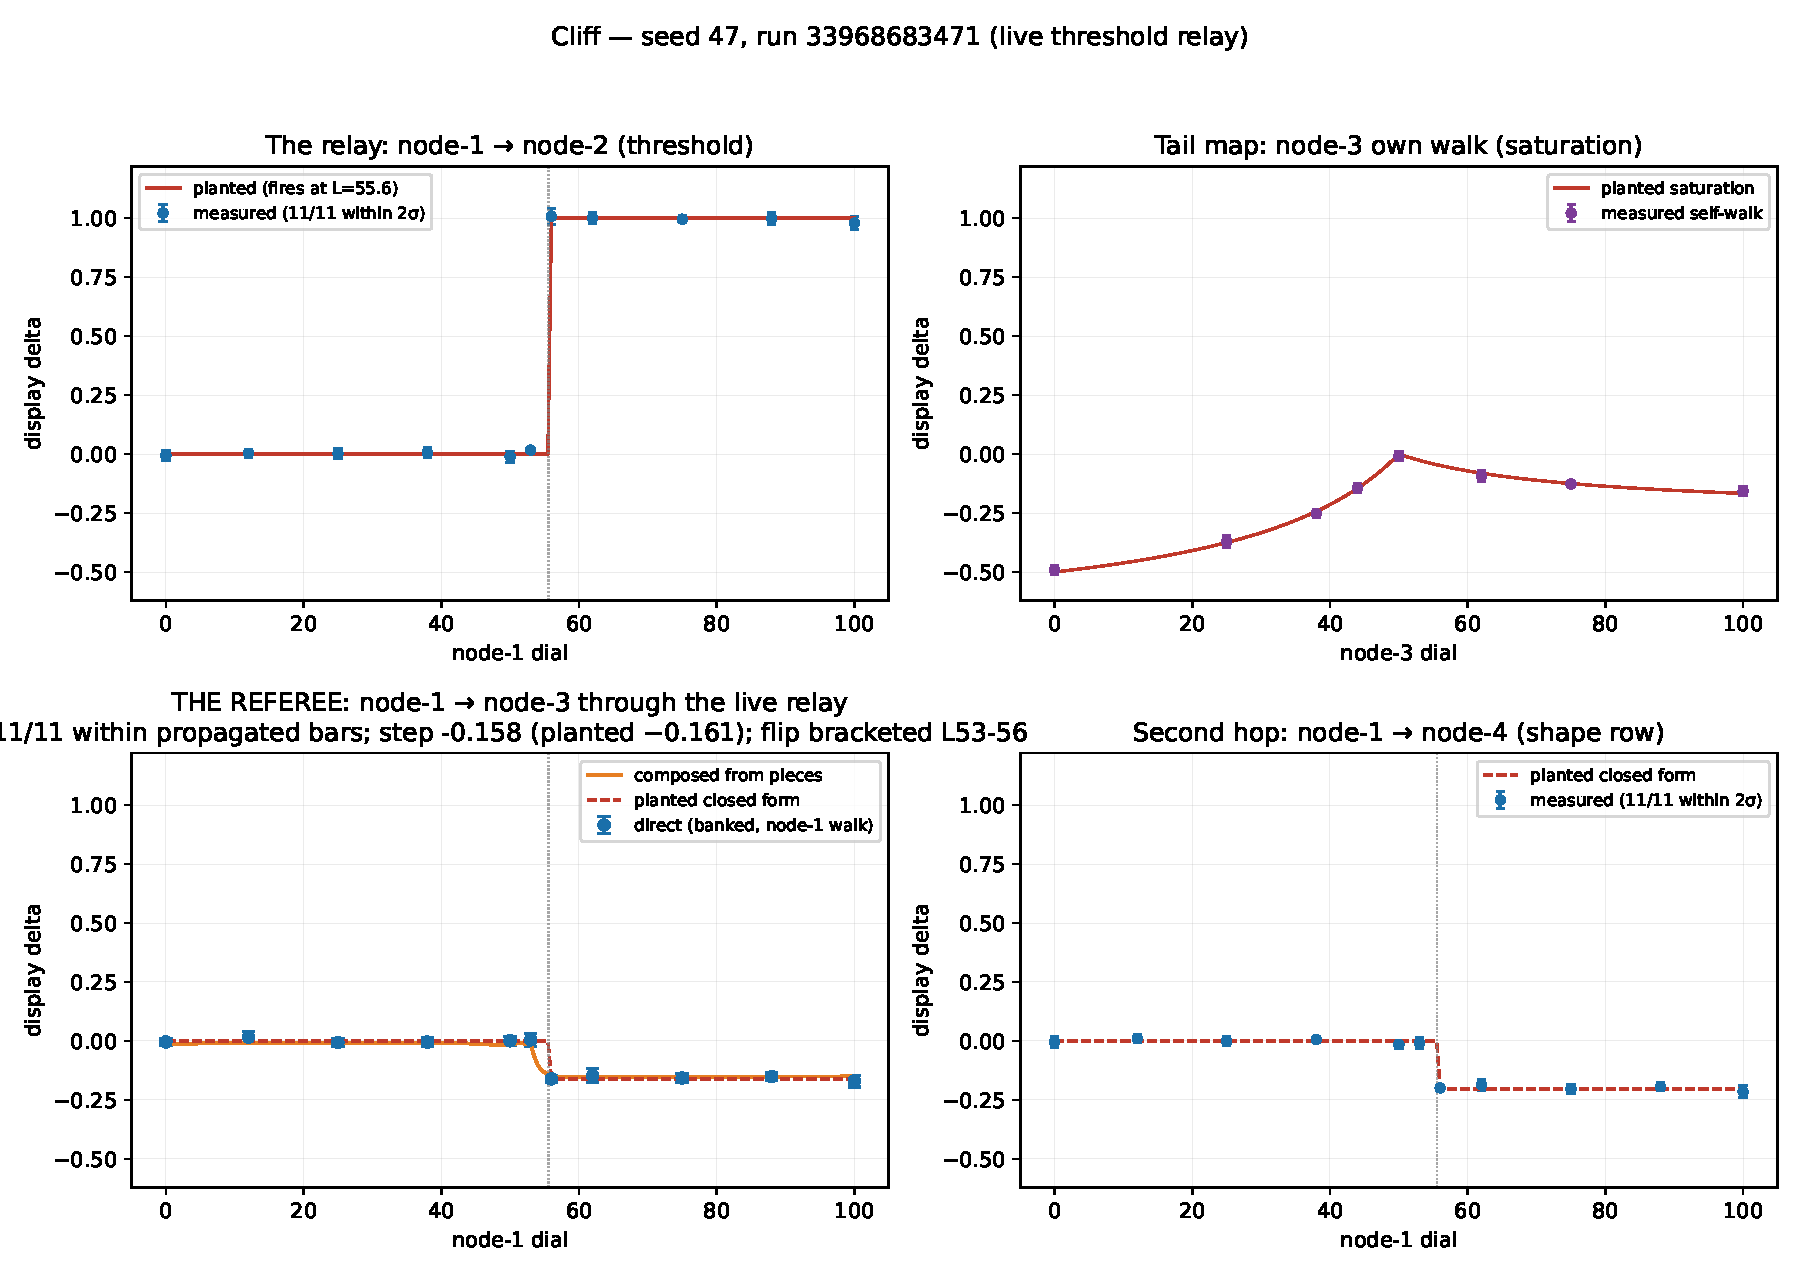
\includegraphics[width=\textwidth]{figures/fig2_cliff_s47.pdf}
\caption{Certification cell, seed 47 (run 33968683471). The relay
piece and tail self-map compose into the far-end prediction
(lower left); the direct walk judges it. Shape row (lower right):
second-hop response against planted closed form.}
\label{fig:cliff47}
\end{figure}

\begin{figure}[t]
\centering
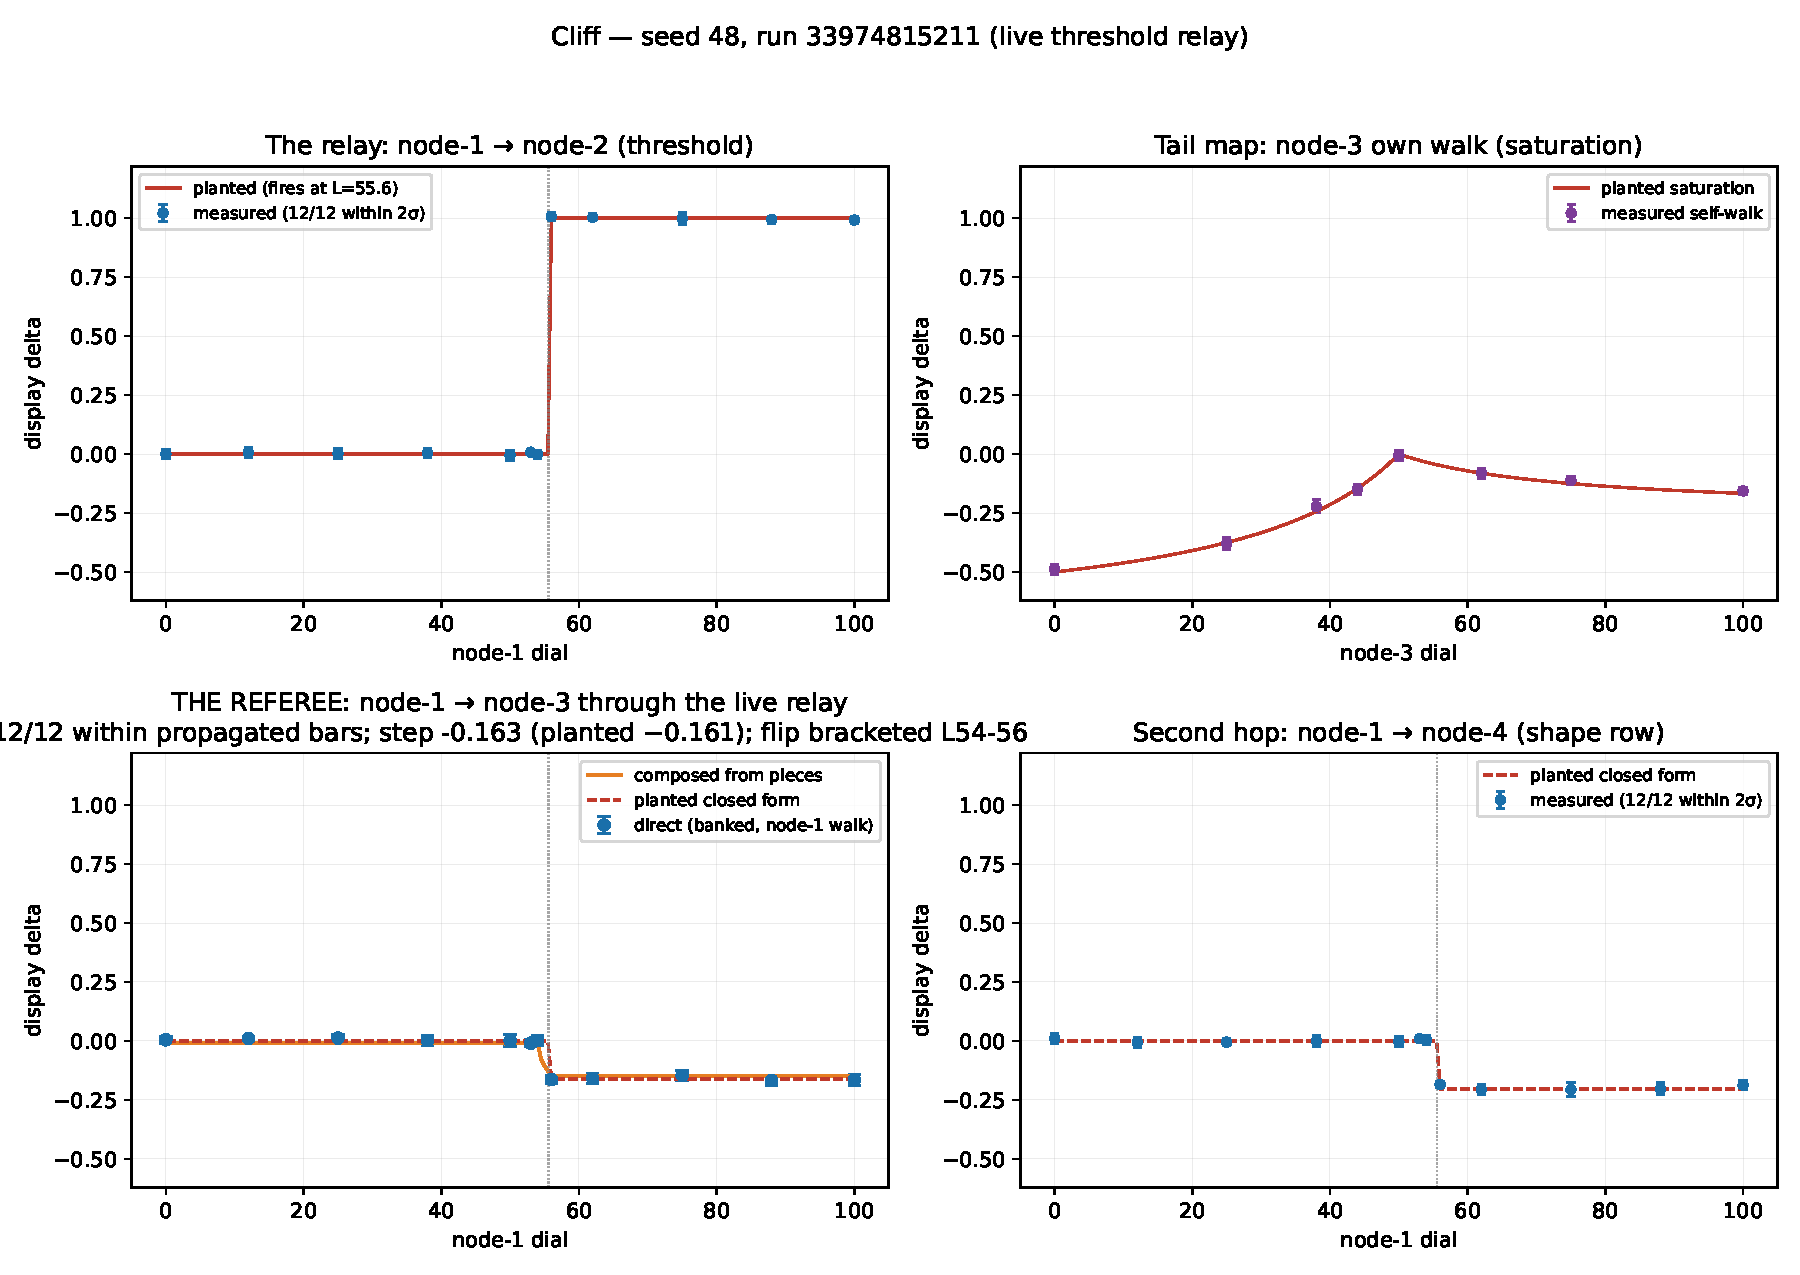
\includegraphics[width=\textwidth]{figures/fig3_cliff_s48.pdf}
\caption{Certification cell, seed 48 (run 33974815211), same design
as Figure~\ref{fig:cliff47}. All panels certify; the flip brackets
one level tighter than seed 47.}
\label{fig:cliff48}
\end{figure}

\subsection{Certification cells: the protocol receipt}
\label{sec:cert}

The two cliff certification cells are the campaign's protocol rows,
run end-to-end on the final build: fair turn-taking with the visible
turn ledger, no timing overrides, terminal close. Both cells complete
all four walkers' maps --- the first four-walker cells in the
campaign's history to do so --- with every curve retired by the priced
stop, and rotation verified event by event from the coordination
trail: 13 lease acquires against 10 quantum yields and 22 denials
(seed 47), strict walker alternation, handovers completing in 3--7
seconds, the waiting walker winning every handover, and every denial
correct (an ex-holder arriving early is refused at the door). The
priced stop's depth allocation is visible in the same record: the
source's walk retires at 11 levels, the tail's at 8, and the node
whose dial moves nothing (planted: no outgoing edges) retires at 6
points of correct flat --- its six points sit within $1.1\sigma$ of
planted zero. A complete four-walker cell costs ${\approx}\,2$ hours
wall-clock.

The scheduler receipt runs through the whole campaign and is worth
stating as one line of method: verdict quality under a defective
scheduler is a lottery --- the starved seed 48 row passed 14/14
\emph{by luck} while the identically starved seed 47 failed 20/22
with both misses localized to the coarse map region --- and the
repair is certified by its own rows, not asserted. The fair-but-thin
row (25/31) then isolated a second defect (the retirement verdict
ignoring the walker's own self-curve), whose repair preceded the two
certification cells above.

\subsection{Shapes, salvage, and the boundary}
\label{sec:salvage}

Three rows complete the campaign's edges. The \emph{poly} rows
validate shape composition on smooth convex nonlinearity: polynomial
piece and saturation-of-polynomial, 12/12 and 12/12 against planted
closed forms, spans thirty and eighteen noise bars. The \emph{salvage}
row is a dead plant --- authored before the pre-flight gate, its
saturation relay can never reach the threshold it was meant to feed
($f_{\text{sat}} \le 0.5$, the fire line, strictly) --- and it
returned two clean receipts anyway: the piece matches its closed form
at 18/18 points, and with prediction identically zero, all 36
downstream points sit within $2\sigma$ of zero. No phantom firing at
the discontinuity the author believed in. The \emph{depth boundary}
row plants three cascaded nonlinear stages: end-to-end response
composes to ${\approx}\,0.001$ --- twenty times below the floor ---
and the direct walk measures faithful flat noise. The referee is
honestly vacuous there, and the boundary is thereby measured: at
$\sigma{=}0.02$ with this door family, composition reaches
${\approx}\,2$ nonlinear hops.

\subsection{The metrology of composed bars}
\label{sec:metrology}

The referee rule~\eqref{eq:referee} prices each comparison with
propagated bars. Its validation is the campaign's quiet headline.
Under the stated rule, 95 of 97 referee points certify (98\%; nominal
for $2\sigma$ is 95.4\%), with median deviation ${\approx}\,0.3\sigma$
--- the bars are honest and slightly conservative, not tuned. Under
the strict variant that ignores the composed side's uncertainty, the
count drops to 91/97: the junction row loses three shelf points
($z$ up to $2.97$ against predictions whose own bars are
${\approx}50\%$ wider than the direct bars there) and cliff seed 48
loses one ($z{=}2.20$ on a thin direct bar). A referee that punished
predictions for uncertainty they had already reported would be
over-rejecting; a referee that never missed would be vacuous. The
observed behavior sits where honest metrology sits.

\section{Boundaries}
\label{sec:boundaries}

We name the limits as measured, without softening.

\emph{Composition horizon.} ${\approx}\,2$ nonlinear hops at
$\sigma{=}0.02$ for this door family. Deeper composition needs
quieter substrates or linear pipes between doors (which reset the
attenuation budget). The horizon is a property of the floor, not of
the arithmetic.

\emph{Memoryless doors.} Every receipt assumes the door answers the
same ask the same way --- no hysteresis, no state. Doors with memory
are the next tier and are untested.

\emph{Continuous inputs.} Levels are continuous dial positions.
Categorical switches (discrete modes) compose differently and are
untested.

\emph{Static world.} The planted substrate is stationary for the
cell's duration. Drift --- edges whose strength moves while the map is
being built --- is the successor question, priced by the map's
refresh economics.

\emph{Bench class.} All evidence is from a mathematical bench with
closed-form truth. No physical substrate appears in this campaign.

\emph{Scheduler provenance.} Rows before the certification cells ran
under earlier protocol builds (timing overrides; pre-ledger
scheduling; a retirement verdict that ignored self-curves). Their
defects are disclosed with their numbers, and the two certification
cells are the rows that carry none of them.

\section{Discussion}
\label{sec:discussion}

\paragraph{Why the horizon makes composition necessary.}
Past two nonlinear hops at this floor, the direct far-end measurement
does not become expensive --- it becomes \emph{meaningless}: the
signal is under the noise and no budget of trials recovers it. The
only route to far-end knowledge is through pieces measured where the
signal is still strong. Composition is therefore not an optimization
of the measurement process; it is the remaining door. The boundary
row makes this concrete rather than rhetorical.

\paragraph{The map as computable self-knowledge.}
A certified, composed coupling map changes what the collecting of
agents can do without new measurements: cascades can be traced
before anyone fires them (``if this sender pushes, who moves, how
much, with what confidence''); attribution questions become lookups;
what-if analysis becomes re-simulation on the map, priced by the
propagated bars. None of this requires the agents to coordinate
beyond the measurement protocol they already run.

\paragraph{Transfer, one paragraph, gated.}
A map measured on one system is a prior for its neighbors. Whether
that prior pays its verification cost is an economics question ---
map half-life against refresh cost --- that drift cells must answer
before transfer is claimed. This paper claims nothing there.

\paragraph{Next rung.}
With detection~\cite{p1}, characterization~\cite{p2}, and composition
in hand, the remaining half of the loop is action: using the composed
map to steer the system toward chosen operating points, with the same
referee discipline (predict, act, film, compare) certifying the
steering claims. That is the successor paper's question, and the
composed bars of this one are its entry ticket.

\section*{Reproducibility}

Every run carries an external identifier (Table~\ref{tab:rows}). The
evidence bundle retains the exported curves with per-point bars, the
node maps, the coordination trails of the certification cells, and the
figure-regeneration script; every figure in this paper regenerates
from that bundle by one command. Verdicts are recomputed from curves,
never read from run badges.

\bibliographystyle{plain}
\bibliography{references}

\end{document}
